% This file is generated by the MATLAB m-file laprint.m. It can be included
% into LaTeX documents using the packages graphicx, color and psfrag.
% It is accompanied by a postscript file. A sample LaTeX file is:
%    \documentclass{article}\usepackage{graphicx,color,psfrag}
%    \begin{document}% This file is generated by the MATLAB m-file laprint.m. It can be included
% into LaTeX documents using the packages graphicx, color and psfrag.
% It is accompanied by a postscript file. A sample LaTeX file is:
%    \documentclass{article}\usepackage{graphicx,color,psfrag}
%    \begin{document}% This file is generated by the MATLAB m-file laprint.m. It can be included
% into LaTeX documents using the packages graphicx, color and psfrag.
% It is accompanied by a postscript file. A sample LaTeX file is:
%    \documentclass{article}\usepackage{graphicx,color,psfrag}
%    \begin{document}% This file is generated by the MATLAB m-file laprint.m. It can be included
% into LaTeX documents using the packages graphicx, color and psfrag.
% It is accompanied by a postscript file. A sample LaTeX file is:
%    \documentclass{article}\usepackage{graphicx,color,psfrag}
%    \begin{document}\input{uavg_eps}\end{document}
% See http://www.mathworks.de/matlabcentral/fileexchange/loadFile.do?objectId=4638
% for recent versions of laprint.m.
%
% created by:           LaPrint version 3.16 (13.9.2004)
% created on:           13-Sep-2019 11:27:25
% eps bounding box:     14.3395 cm x 10.7546 cm
% comment:              
%
\begin{psfrags}%
\psfragscanon%
%
% text strings:
\psfrag{s02}[b][b]{\color[rgb]{0.15,0.15,0.15}\setlength{\tabcolsep}{0pt}\begin{tabular}{c}$\overline{v}^+$\end{tabular}}%
\psfrag{s04}[][]{\color[rgb]{0,0,0}\setlength{\tabcolsep}{0pt}\begin{tabular}{c}(a)\end{tabular}}%
\psfrag{s05}[t][t]{\color[rgb]{0.15,0.15,0.15}\setlength{\tabcolsep}{0pt}\begin{tabular}{c}$x^+$\end{tabular}}%
%
% axes ticklabel color:
\color[rgb]{0.15,0.15,0.15}%
%
% xticklabels:
\psfrag{x01}[t][t]{$10^{10^{-1}}$}%
\psfrag{x02}[t][t]{$10^{10^{0}}$}%
\psfrag{x03}[t][t]{$10^{10^{1}}$}%
\psfrag{x04}[t][t]{$10^{10^{2}}$}%
\psfrag{x05}[t][t]{$10^{10^{3}}$}%
%
% yticklabels:
\psfrag{v01}[r][r]{0}%
\psfrag{v02}[r][r]{5}%
\psfrag{v03}[r][r]{10}%
\psfrag{v04}[r][r]{15}%
\psfrag{v05}[r][r]{20}%
\psfrag{v06}[r][r]{25}%
%
% Figure:
\resizebox{14.3395cm}{!}{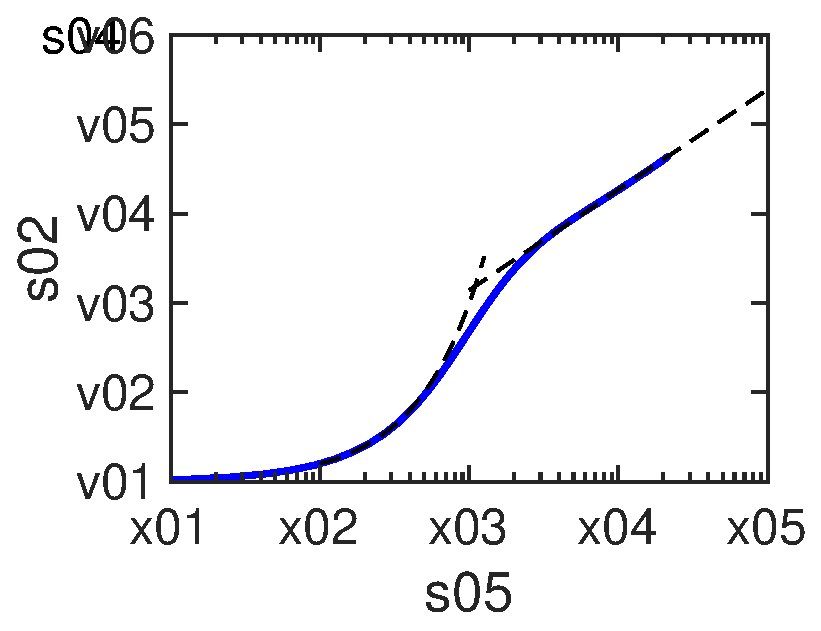
\includegraphics{uavg_eps.eps}}%
\end{psfrags}%
%
% End uavg_eps.tex
\end{document}
% See http://www.mathworks.de/matlabcentral/fileexchange/loadFile.do?objectId=4638
% for recent versions of laprint.m.
%
% created by:           LaPrint version 3.16 (13.9.2004)
% created on:           13-Sep-2019 11:27:25
% eps bounding box:     14.3395 cm x 10.7546 cm
% comment:              
%
\begin{psfrags}%
\psfragscanon%
%
% text strings:
\psfrag{s02}[b][b]{\color[rgb]{0.15,0.15,0.15}\setlength{\tabcolsep}{0pt}\begin{tabular}{c}$\overline{v}^+$\end{tabular}}%
\psfrag{s04}[][]{\color[rgb]{0,0,0}\setlength{\tabcolsep}{0pt}\begin{tabular}{c}(a)\end{tabular}}%
\psfrag{s05}[t][t]{\color[rgb]{0.15,0.15,0.15}\setlength{\tabcolsep}{0pt}\begin{tabular}{c}$x^+$\end{tabular}}%
%
% axes ticklabel color:
\color[rgb]{0.15,0.15,0.15}%
%
% xticklabels:
\psfrag{x01}[t][t]{$10^{10^{-1}}$}%
\psfrag{x02}[t][t]{$10^{10^{0}}$}%
\psfrag{x03}[t][t]{$10^{10^{1}}$}%
\psfrag{x04}[t][t]{$10^{10^{2}}$}%
\psfrag{x05}[t][t]{$10^{10^{3}}$}%
%
% yticklabels:
\psfrag{v01}[r][r]{0}%
\psfrag{v02}[r][r]{5}%
\psfrag{v03}[r][r]{10}%
\psfrag{v04}[r][r]{15}%
\psfrag{v05}[r][r]{20}%
\psfrag{v06}[r][r]{25}%
%
% Figure:
\resizebox{14.3395cm}{!}{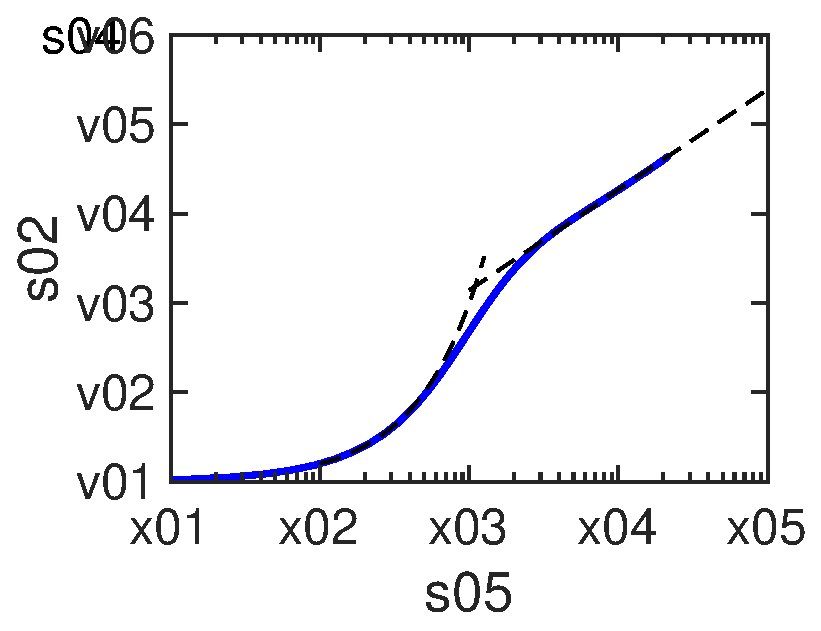
\includegraphics{uavg_eps.eps}}%
\end{psfrags}%
%
% End uavg_eps.tex
\end{document}
% See http://www.mathworks.de/matlabcentral/fileexchange/loadFile.do?objectId=4638
% for recent versions of laprint.m.
%
% created by:           LaPrint version 3.16 (13.9.2004)
% created on:           13-Sep-2019 11:27:25
% eps bounding box:     14.3395 cm x 10.7546 cm
% comment:              
%
\begin{psfrags}%
\psfragscanon%
%
% text strings:
\psfrag{s02}[b][b]{\color[rgb]{0.15,0.15,0.15}\setlength{\tabcolsep}{0pt}\begin{tabular}{c}$\overline{v}^+$\end{tabular}}%
\psfrag{s04}[][]{\color[rgb]{0,0,0}\setlength{\tabcolsep}{0pt}\begin{tabular}{c}(a)\end{tabular}}%
\psfrag{s05}[t][t]{\color[rgb]{0.15,0.15,0.15}\setlength{\tabcolsep}{0pt}\begin{tabular}{c}$x^+$\end{tabular}}%
%
% axes ticklabel color:
\color[rgb]{0.15,0.15,0.15}%
%
% xticklabels:
\psfrag{x01}[t][t]{$10^{10^{-1}}$}%
\psfrag{x02}[t][t]{$10^{10^{0}}$}%
\psfrag{x03}[t][t]{$10^{10^{1}}$}%
\psfrag{x04}[t][t]{$10^{10^{2}}$}%
\psfrag{x05}[t][t]{$10^{10^{3}}$}%
%
% yticklabels:
\psfrag{v01}[r][r]{0}%
\psfrag{v02}[r][r]{5}%
\psfrag{v03}[r][r]{10}%
\psfrag{v04}[r][r]{15}%
\psfrag{v05}[r][r]{20}%
\psfrag{v06}[r][r]{25}%
%
% Figure:
\resizebox{14.3395cm}{!}{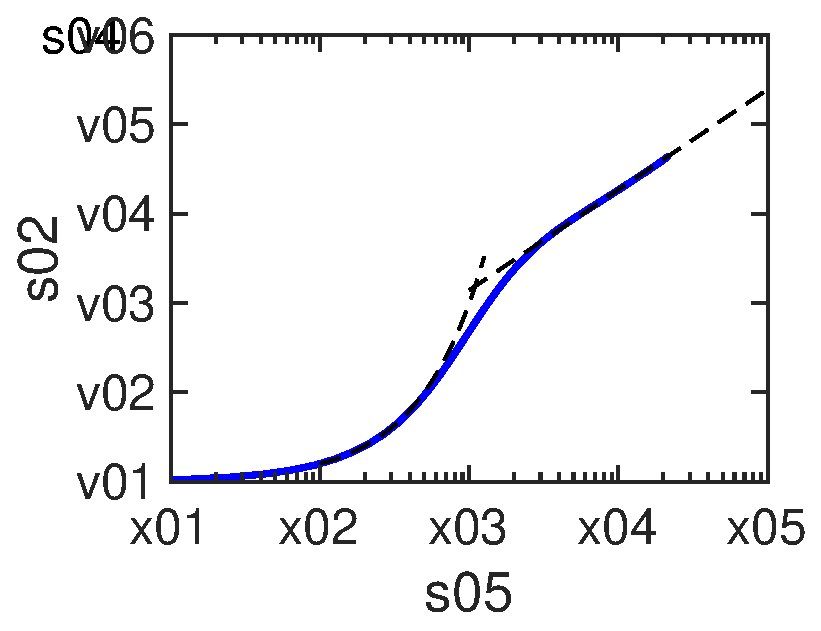
\includegraphics{uavg_eps.eps}}%
\end{psfrags}%
%
% End uavg_eps.tex
\end{document}
% See http://www.mathworks.de/matlabcentral/fileexchange/loadFile.do?objectId=4638
% for recent versions of laprint.m.
%
% created by:           LaPrint version 3.16 (13.9.2004)
% created on:           13-Sep-2019 11:27:25
% eps bounding box:     14.3395 cm x 10.7546 cm
% comment:              
%
\begin{psfrags}%
\psfragscanon%
%
% text strings:
\psfrag{s02}[b][b]{\color[rgb]{0.15,0.15,0.15}\setlength{\tabcolsep}{0pt}\begin{tabular}{c}$\overline{v}^+$\end{tabular}}%
\psfrag{s04}[][]{\color[rgb]{0,0,0}\setlength{\tabcolsep}{0pt}\begin{tabular}{c}(a)\end{tabular}}%
\psfrag{s05}[t][t]{\color[rgb]{0.15,0.15,0.15}\setlength{\tabcolsep}{0pt}\begin{tabular}{c}$x^+$\end{tabular}}%
%
% axes ticklabel color:
\color[rgb]{0.15,0.15,0.15}%
%
% xticklabels:
\psfrag{x01}[t][t]{$10^{10^{-1}}$}%
\psfrag{x02}[t][t]{$10^{10^{0}}$}%
\psfrag{x03}[t][t]{$10^{10^{1}}$}%
\psfrag{x04}[t][t]{$10^{10^{2}}$}%
\psfrag{x05}[t][t]{$10^{10^{3}}$}%
%
% yticklabels:
\psfrag{v01}[r][r]{0}%
\psfrag{v02}[r][r]{5}%
\psfrag{v03}[r][r]{10}%
\psfrag{v04}[r][r]{15}%
\psfrag{v05}[r][r]{20}%
\psfrag{v06}[r][r]{25}%
%
% Figure:
\resizebox{14.3395cm}{!}{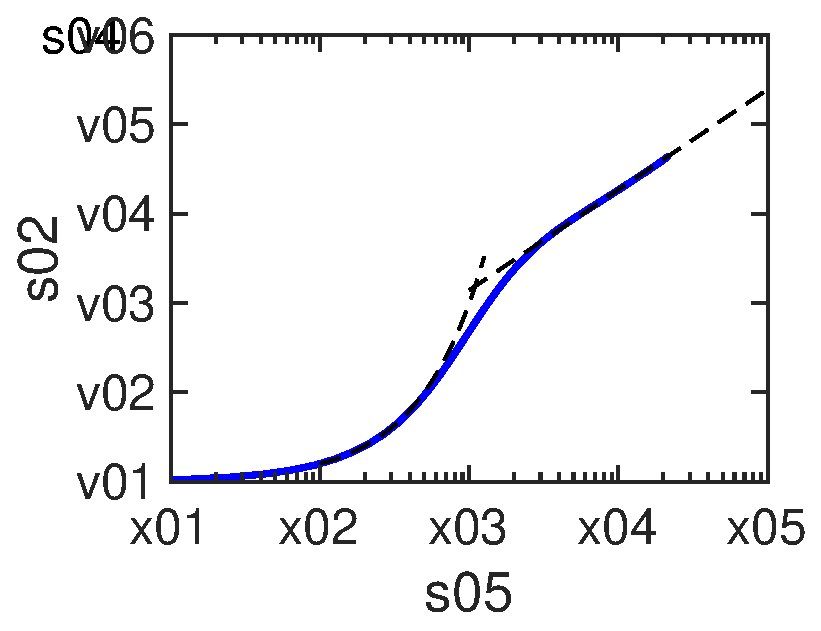
\includegraphics{uavg_eps.eps}}%
\end{psfrags}%
%
% End uavg_eps.tex
